\documentclass[]{article}
\usepackage{lmodern}
\usepackage{amssymb,amsmath}
\usepackage{ifxetex,ifluatex}
\usepackage{fixltx2e} % provides \textsubscript
\ifnum 0\ifxetex 1\fi\ifluatex 1\fi=0 % if pdftex
  \usepackage[T1]{fontenc}
  \usepackage[utf8]{inputenc}
\else % if luatex or xelatex
  \ifxetex
    \usepackage{mathspec}
  \else
    \usepackage{fontspec}
  \fi
  \defaultfontfeatures{Ligatures=TeX,Scale=MatchLowercase}
\fi
% use upquote if available, for straight quotes in verbatim environments
\IfFileExists{upquote.sty}{\usepackage{upquote}}{}
% use microtype if available
\IfFileExists{microtype.sty}{%
\usepackage{microtype}
\UseMicrotypeSet[protrusion]{basicmath} % disable protrusion for tt fonts
}{}
\usepackage[margin=1in]{geometry}
\usepackage{hyperref}
\hypersetup{unicode=true,
            pdftitle={Chapter Two},
            pdfauthor={Ryan B. Honea},
            pdfborder={0 0 0},
            breaklinks=true}
\urlstyle{same}  % don't use monospace font for urls
\usepackage{longtable,booktabs}
\usepackage{graphicx,grffile}
\makeatletter
\def\maxwidth{\ifdim\Gin@nat@width>\linewidth\linewidth\else\Gin@nat@width\fi}
\def\maxheight{\ifdim\Gin@nat@height>\textheight\textheight\else\Gin@nat@height\fi}
\makeatother
% Scale images if necessary, so that they will not overflow the page
% margins by default, and it is still possible to overwrite the defaults
% using explicit options in \includegraphics[width, height, ...]{}
\setkeys{Gin}{width=\maxwidth,height=\maxheight,keepaspectratio}
\IfFileExists{parskip.sty}{%
\usepackage{parskip}
}{% else
\setlength{\parindent}{0pt}
\setlength{\parskip}{6pt plus 2pt minus 1pt}
}
\setlength{\emergencystretch}{3em}  % prevent overfull lines
\providecommand{\tightlist}{%
  \setlength{\itemsep}{0pt}\setlength{\parskip}{0pt}}
\setcounter{secnumdepth}{0}
% Redefines (sub)paragraphs to behave more like sections
\ifx\paragraph\undefined\else
\let\oldparagraph\paragraph
\renewcommand{\paragraph}[1]{\oldparagraph{#1}\mbox{}}
\fi
\ifx\subparagraph\undefined\else
\let\oldsubparagraph\subparagraph
\renewcommand{\subparagraph}[1]{\oldsubparagraph{#1}\mbox{}}
\fi

%%% Use protect on footnotes to avoid problems with footnotes in titles
\let\rmarkdownfootnote\footnote%
\def\footnote{\protect\rmarkdownfootnote}

%%% Change title format to be more compact
\usepackage{titling}

% Create subtitle command for use in maketitle
\newcommand{\subtitle}[1]{
  \posttitle{
    \begin{center}\large#1\end{center}
    }
}

\setlength{\droptitle}{-2em}
  \title{Chapter Two}
  \pretitle{\vspace{\droptitle}\centering\huge}
  \posttitle{\par}
  \author{Ryan B. Honea}
  \preauthor{\centering\large\emph}
  \postauthor{\par}
  \date{}
  \predate{}\postdate{}


\begin{document}
\maketitle

\subsection{Exercise One}\label{exercise-one}

\paragraph{Question}\label{question}

Genetically similar seeds are randomly assigned to be raised in either a
nutritionally entriched environment (treatment group) or standard
conditions (control group) usig a completely randomized experimental
design. After a predetermined time, all plants are harvested, dried and
weighed. The results, expressed in grams, for 20 plants in each group
are shown in the table below.

\begin{center}
\begin{tabular}{@{}cccc@{}}
\toprule
\multicolumn{2}{c}{Treatment Group} & \multicolumn{2}{c}{Control Group} \\ \midrule
4.81             & 5.36             & 4.17            & 4.66            \\
4.17             & 3.48             & 3.05            & 5.58            \\
4.41             & 4.69             & 5.18            & 3.66            \\
3.59             & 4.44             & 4.01            & 4.50            \\
5.87             & 4.89             & 6.11            & 3.90            \\
3.83             & 4.71             & 4.10            & 4.61            \\
6.03             & 5.48             & 5.17            & 5.62            \\
4.98             & 4.32             & 3.57            & 4.53            \\
4.90             & 5.15             & 5.33            & 6.05            \\
5.75             & 6.34             & 5.59            & 5.14            \\ \bottomrule
\end{tabular}
\end{center}

We want to test whether there is any difference in yield between the two
groups. Let \(Y_{jk}\) denote the \(k\)th observation in the \(j\)th
group where \(j = 1\) for the treatment group, \(j = 2\) for the control
group and \(k = 1,...,20\) for both groups. Assume that the \(Y_{jk}\)'s
are independent random variables with
\(Y_{jk} \sim \text{N}(\mu_j, \sigma^2)\). The null hypothesis
\(H_0: \mu_1 = \mu_2 = \mu\), that there is no differenc, is to be
compared with the alternative hypothesis \(H_1 : \mu_1 \neq \mu_2\).

\subsubsection{Solution}\label{solution}

\textbf{(a):} Conduct a exploratory analysis of the data looking at the
distributions for each group (e.g.~using dot plots, stem and leaf plots
or Normal probability plots) and calculate summary statistics (e.g.,
means, medians, standard derivations, maxima and minima). What can you
infer from these investigations?

\emph{Solution: } We begin by making a histogram of the joint data from
treatment and control, followed by an Anderson Darling test to assess
the normality of the joint set of data.

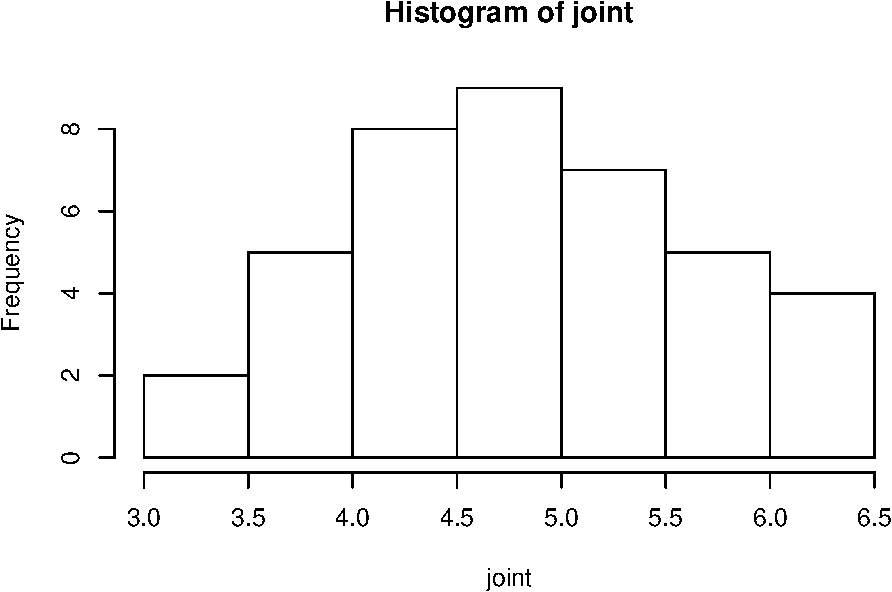
\includegraphics{ExercisesWithSolutions_files/figure-latex/unnamed-chunk-2-1.pdf}

\begin{verbatim}
## 
##  Shapiro-Wilk normality test
## 
## data:  joint
## W = 0.98419, p-value = 0.8387
\end{verbatim}

With a \(p\)-value of .84, we can assume this data behaves normally
(which the histogram also seems to indicate). We now find the mean and
standard deviations of the treatment and control vectors.

\begin{verbatim}
## Mean of treatment:  4.8555 
## Standard Deviation of treatment:  0.7904594
\end{verbatim}

\begin{verbatim}
## 
## Mean of control:  4.7265 
## Standard Deviation of control:  0.8635257
\end{verbatim}

The initial assumption is that these means are not significiantly
different, but that will potentially be confirmed in later tests.

\textbf{(b):} Perform an unpaired t-test on these data and calculate a
95\% confidence interval for the difference between the group means.
Interpret these results.

\emph{Solution: }

\begin{verbatim}
## 
##  Welch Two Sample t-test
## 
## data:  treatment and control
## t = 0.49279, df = 37.707, p-value = 0.625
## alternative hypothesis: true difference in means is not equal to 0
## 95 percent confidence interval:
##  -0.4010672  0.6590672
## sample estimates:
## mean of x mean of y 
##    4.8555    4.7265
\end{verbatim}

The results of this t-test suggest that there is so significant
statistical difference between the means. With a confidence interval
that includes 0, this is especially clear.

\textbf{(c):} The following models can be used to test the null
hypothesis \(H_0\) against the alternative hypothesis \(H_1\), where

\begin{align*}
H_0 : E(Y_{jk}) &= \mu;\quad Y_{jk} \sim \text{N}(\mu, \sigma^2),\\
H_1 : E(Y_{jk}) &= \mu_j;\quad Y_{jk} \sim \text{N}(\mu_j, \sigma^2),
\end{align*}

for \(j = 1,2\) and \(k = 1,...,20\). Find the maximum likelihood and
least squares estimate of the parameters \(\mu, \mu_1, \mu_2\) assuming
\(\sigma^2\) is a known constant.

\emph{Solution: }We begin by utilizing the most-likely estimate. Note
the following probability density functions.

\begin{align*}
f(\mu; Y_{jk}) &= \frac{1}{\sqrt{2\pi\sigma^2}}\exp\left(-\frac{(Y_{jk} - \mu)^2}{2\sigma^2} \right)\\
f(\mu_1; Y_{1k}) &= \frac{1}{\sqrt{2\pi\sigma^2}}\exp\left(-\frac{(Y_{jk} - \mu_1)^2}{2\sigma^2} \right)\\
f(\mu_2; Y_{2k}) &= \frac{1}{\sqrt{2\pi\sigma^2}}\exp\left(-\frac{(Y_{jk} - \mu_2)^2}{2\sigma^2} \right)
\end{align*}

Using the log-likelihood, we have the following formulas

\begin{align*}
l_0 &= \frac{1}{2}\sum_{j = 1}^2\sum_{k=1}^{20}\left[\log(2\pi\sigma^2) - \frac{1}{2\sigma^2}(Y_{jk} - \mu)^2\right] & &= 20\log(2\pi\sigma^2) - \frac{1}{2\sigma^2}\sum_{j = 1}^2\sum_{k=1}^{20}(Y_{jk} - \mu)^2\\
l_1 &= \frac{1}{2}\sum_{j = 1}^2\sum_{k=1}^{20}\left[\log(2\pi\sigma^2) - \frac{1}{2\sigma^2}(Y_{jk} - \mu_j)^2\right] & &= 20\log(2\pi\sigma^2) - \frac{1}{2\sigma^2}\left(\sum_{k=1}^{20}(Y_{1k} - \mu_1)^2 + \sum_{k=1}^{20}(Y_{2k}-\mu_2)^2 \right)
\end{align*}

When taking the derivatives in respect to \(\mu, \mu_1,\) and \(\mu_2\)
and setting them to zero, we gain

\begin{align*}
\frac{\partial l_0}{\partial \mu} &= \frac{1}{\sigma^2}\sum_{j = 1}^2\sum_{k=1}^{20}(Y_{jk} - \mu) = 0      \\
& \implies \sum_{j=1}^2\sum_{k=1}^{20}Y_{jk} - 40\mu = 0\\
& \implies \mu_{MLE} = \dfrac{\sum_{j=1}^2\sum_{k=1}^{20}Y_{jk}}{40}
\end{align*}\begin{align*}
\frac{\partial l_1}{\partial \mu_1} &= \frac{1}{\sigma^2}\sum_{k=1}^{20}(Y_{1k} - \mu_1) = 0     &
\frac{\partial l_1}{\partial \mu_2} &= \frac{1}{\sigma^2}\sum_{k=1}^{20}(Y_{2k} - \mu_2) = 0\\
& \implies \mu_{1MLE} = \dfrac{\sum_{k=1}^{20}Y_{1k}}{20} & 
& \implies \mu_{2MLE} = \dfrac{\sum_{k=1}^{20}Y_{2k}}{20}
\end{align*}

These all result in the sample means. The least squares estimates result
in the same below.

\begin{align*}
S_0 &= \sum_{j=1}^2\sum_{k=1}^{20}(Y_{jk} - \mu)\\
S_1 &= \sum_{k=1}^{20}(Y_{1k} - \mu_1)^2 + \sum_{k=1}^{20}(Y_{2k}-\mu_2)^2
\end{align*}

Similar to the MLE, we take the derivative of these in respect to
\(\mu, \mu_1,\) and \(\mu_2\) and set them to zero to find the best
estimates.

\begin{align*}
\frac{\partial S_0}{\partial \mu} & = -2\sum_{j=1}^2\sum_{k=1}^{20}(Y_{jk} - \mu) = 0\\
& \implies \sum_{j=1}^2\sum_{k=1}^{20}Y_{jk} = 40\mu \\
& \implies \mu = \dfrac{\sum_{j=1}^2\sum_{k=1}^{20}Y_{jk}}{40}
\end{align*}\begin{align*}
\frac{\partial S_1}{\partial \mu_1} &= -2\sum_{k=1}^{20}(Y_{1k} - \mu_1) = 0 & 
\frac{\partial S_1}{\partial \mu_2} &= -2\sum_{k=1}^{20}(Y_{2k} - \mu_2) = 0\\
& \implies \mu_{1LSE} = \dfrac{\sum_{k=1}^{20}Y_{1k}}{20} &
& \implies \mu_{2LSE} = \dfrac{\sum_{k=1}^{20}Y_{2k}}{20}
\end{align*}

\textbf{(d):} Show that the minimum values of the least squares criteria
are

\begin{align*}
\text{for } H_0, \quad \hat{S_0} &=  \sum \sum (Y_{jk} - \overline{Y})^2, \text{ where } \overline{Y} = \sum_{j=1}^2\sum_{k=1}^K Y_{jk}/40;\\
\text{for } H_1, \quad \hat{S_1} &= \sum \sum (Y_{jk} - \overline{Y_j})^2, \text{ where } \overline{Y_j} = \sum_{k=1}^K Y_{jk}/20;
\end{align*}

for \(j = 1,2\).

\emph{Solution: }From \textbf{(c)}, we know that the

\begin{align*}
\frac{\partial S_0}{\partial \mu} & = -2\sum_{j=1}^2\sum_{k=1}^{20}(Y_{jk} - \mu)\\
\frac{\partial S_1}{\partial \mu_j} &= -2\sum_{k=1}^{20}(Y_{jk} - \mu_j)
\end{align*}

The estimates that resulted from these are equivelant to
\(\overline{Y}\) and \(\overline{Y_j}\). If it can be shown that the
second derivative is positive, then we know that these are the minimum
values for \(\hat{S_0}\) and \(\hat{S_1}\).

\begin{align*}
\frac{\partial^2 S_0}{\partial \mu^2} &= 2 & 
\frac{\partial^2 S_1}{\partial \mu_j^2} &= 2
\end{align*}

As they are positive, then we know that \(\hat{S_0}\) and \(\hat{S_1}\)
are minimized.

\textbf{(e):} Using the results of Exercise 1.4 show that \[
\frac{1}{\sigma^2}\hat{S_1} = \frac{1}{\sigma^2}\sum_{j=1}^2\sum_{k=1}^{20}(Y_{jk} - \mu_j)^2 - \frac{20}{\sigma^2}\sum^{20}_{k=1}(\overline{Y_j} - \mu_j)^2,
\] and deduce that if \(H_1\) is true \[
\frac{1}{\sigma^2}\hat{S_1} \sim \chi^2(38).
\] Similarly show that \[
\frac{1}{\sigma^2}\hat{S_0} = \frac{1}{\sigma^2}\sum_{j=1}^2\sum_{k=1}^{20}(Y_{jk} - \mu)^2 - \frac{40}{\sigma^2}\sum_{j=1}^2(\overline{Y} - \mu)^2
\] and if \(H_0\) is true then \[
\frac{1}{\sigma^2}\hat{S_0} \sim \chi^2(39).
\]

\emph{Solution: } (Note that handwaving is definitely occurring here)
From Exercise 1.4, we know that \[
\sum_{i=1}^n(Y_i - \overline{Y})^2 = \sum_{i=1}^n(Y_i - \mu)^2 - n(\overline{Y} - \mu)^2
\] Similarly, in this case where \(n = K\), we have the following: \[
\hat{S_0} = \sum_{j=1}^2\sum_{k=1}^{20}(Y_{jk} - \overline{Y})^2 = \sum_{j=1}^2\left[\sum_{k=1}^{20}(Y_{jk} - \mu)^2 - 20(\overline{Y} - \mu)^2\right]
\] and \[
\hat{S_1} = \sum_{j=1}^2\sum_{k=1}^{20}(Y_{jk} - \overline{Y_j})^2 = \sum_{j=1}^2\left[\sum_{k=1}^{20}(Y_{jk} - \mu_j)^2 - 20(\overline{Y_j} - \mu_j)^2\right]
\] which with the \(\frac{1}{\sigma^2}\) term will become below

\begin{align*}
\frac{1}{\sigma^2}\hat{S_0} &= \frac{1}{\sigma^2}\sum_{j=1}^2\sum_{k=1}^{20}(Y_{jk} - \mu)^2 - \frac{40}{\sigma^2}\sum_{j=1}^2(\overline{Y} - \mu)^2\\
\frac{1}{\sigma^2}\hat{S_1} &= \frac{1}{\sigma^2}sum_{j=1}^2\sum_{k=1}^{20}(Y_{jk} - \mu_j)^2 - \frac{20}{\sigma^2}\sum^{20}_{k=1}(\overline{Y_j} - \mu_j)^2 \\
\end{align*}

In the case of \(S_0\), we only estimate one parameter, so
\(S_0/\sigma^2 \sim \chi^2(JK - 1)\), while for \(S_0\) we estimate two
parameters so \(S_1/\sigma^2 \sim \chi^2(JK - 2)\). Therefore

\begin{align*}
S_0/\sigma^2 &\sim \chi^2(39)\\
S_1/\sigma^2 &\sim \chi^2(38)\\
\end{align*}

\textbf{(f):} Use an argument similar to the one in Example 2.2.2 and
the results from (e) to deduce that the statistic \[ 
F = \frac{\hat{S_0} - \hat{S_1}}{\hat{S_1}/38}
\] has the central \(F\)-distribution \(F(1,38)\) if \(H_0\) is true and
a non-central distribution if \(H_0\) is not true.

\emph{Solution: }If \(H_0\) is correct, that is the means of the control
and treatment are equal (and so difference is approximately 0 and thus
centralized), then
\(\frac{1}{\sigma^2}(\hat{S_0} - \hat{S_1}) \sim \chi^2(1)\). If \(H_0\)
is not correct, however, then
\(\frac{1}{\sigma^2}(\hat{S_0} - \hat{S_1})\) is not centralized and
cannot be compared and so we use \(S_1\) with it's central chi-squared
distribution. This results in \[
\dfrac{(\hat{S_0} - \hat{S_1})/1}{\hat{S_1}/38} \sim F(1,38)
\] \textbf{(g):} Calculate the \(F\)-statistic from (f) and use it to
test \(H_0\) against \(H_1\). What do you conclude?

\begin{verbatim}
## The F-Statistic is  0.2428452
\end{verbatim}

\begin{verbatim}
## 
## The p-value is  0
\end{verbatim}

\textbf{(h):} Compare the value of \(F\)-statistic from (g) with the
t-statistic from (b), recalling the relationship between the
\(t\)-distribution and the \(F\)-distribution (see Section 1.4.4). Also
compare the conclusion from (b) and (g).

\emph{Solution: }The \(p\)-value from the F-test was \(\approx .75\)
while the \(p\)-value from the t-test was \(\approx .65\). The
\(t\)-statistic was \(\approx .50\) while the \(F\)-statistic was
\(\approx .25\). This makes sense because \(T^2 \sim F(1,40)\) which is
close to the final distribution, and \(T^2 \approx .25\).

\textbf{(i):} Calculate residuals from the model for \(H_0\) and use
them to explore the distributional assumptions.

\emph{Solution: }

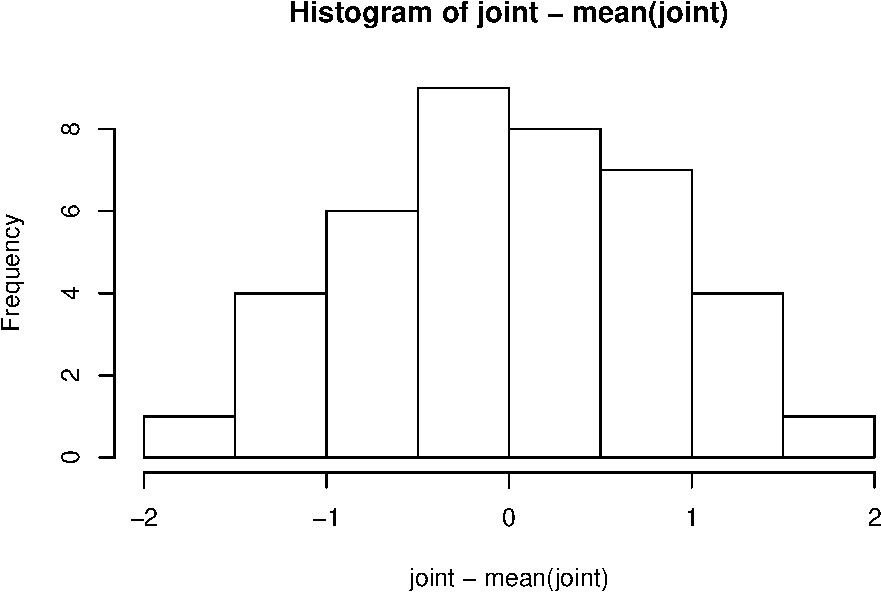
\includegraphics{ExercisesWithSolutions_files/figure-latex/unnamed-chunk-6-1.pdf}

\begin{verbatim}
## 
##  Shapiro-Wilk normality test
## 
## data:  joint - mean(joint)
## W = 0.98419, p-value = 0.8387
\end{verbatim}

Part of the assumption of the normal distribution is the normality of
the residuals, and they indeed distributed approximately normally which
is confirmed by the shapiro test and histogram.

\subsection{Exercise Two}\label{exercise-two}

\paragraph{Question}\label{question-1}

The weights, in kilograms, of twenty men before and after participation
in a ``waist loss'' program are shown in Table 2.8 (Egger et al. 1999).
We want to know if, on average, they retain a weight loss twelve months
after the program.

\begin{center}
\begin{tabular}{@{}ccccccc@{}}
\toprule
Man & Before & After &  & Man & Before & After \\ \cmidrule(r){1-3} \cmidrule(l){5-7} 
1   & 100.8  & 97    &  & 11  & 105    & 105   \\
2   & 102    & 107.5 &  & 12  & 85     & 82.4  \\
3   & 105.9  & 97    &  & 13  & 107.2  & 98.2  \\
4   & 108    & 108   &  & 14  & 80     & 83.6  \\
5   & 92     & 84    &  & 15  & 115.1  & 115   \\
6   & 116.7  & 111.5 &  & 16  & 103.5  & 103   \\
7   & 110.2  & 102.5 &  & 17  & 82     & 80    \\
8   & 135    & 127.5 &  & 18  & 101.5  & 101.5 \\
9   & 123.5  & 118.5 &  & 19  & 103.5  & 102.6 \\
10  & 95     & 94.2  &  & 20  & 93     & 93    \\ \bottomrule
\end{tabular}
\end{center}

Let \(Y_{jk}\) denote the weight of the \(k\)th man at the \(j\)th time,
where \(j = 1\) before the program and \(j = 2\) twelve months later.
Assume the \(Y_{jk}\)'s are independent random variables
\(Y_{jk} \sim N(\mu_j, \sigma^2)\) for \(j = 1,2\) and \(k = 1,...,20\).

\textbf{(a):} Use an unpaired t-test to test the hypothesis \[
H_0 : \mu_1 = \mu_2 \quad \text{versus} \quad H_1: \mu_1 \neq \mu_2.
\]

\emph{Solution: } I'll begin by entering the data into R.

\begin{verbatim}
## 
##  Welch Two Sample t-test
## 
## data:  before and after
## t = 0.65471, df = 37.749, p-value = 0.5166
## alternative hypothesis: true difference in means is not equal to 0
## 95 percent confidence interval:
##  -5.639874 11.029874
## sample estimates:
## mean of x mean of y 
##   103.295   100.600
\end{verbatim}

\textbf{(b):} Let \(D_k = Y_{1k} - Y_{2k}\), for \(k = 1,...,20\).
Formulate models for testing \(H_0\) against \(H_1\) using the
\(D_k\)'s. Using analogous methods to Exercise 2.1 above, assuming
\(\sigma^2\) is a known constant, test \(H_0\) against \(H_1\).

Unsure where to go from here.

\textbf{(c):} The analysis in (b) is a paired t-test which uses the
natural relationship between weights of the \emph{same} person before
and after the program. Are the conclusions the same from (a) and (b)?

Unsure where to go from here.

\textbf{(d):} List the assumptions made for (a) and (b). Which analysis
is more appropriate for these data?

Unsure where to go from here.

\pagebreak
\#\# Exercise Three \#\#\#\# Question For model (2.7) for the data on
birthweight and gestational age, using methods similar to those for
Exercise 1.4, show

\begin{align*}
\hat{S_1} &= \sum_{j=1}^J\sum_{k=1}^K(Y_{jk} - a_j - b_jx_{jk})^2\\
&= \sum_{j=1}^J\sum_{k=1}^K[(Y_{jk} - (a_j + \beta_jx_{jk})]^2 - K\sum_{j=1}^J(\overline{Y_j} - \alpha_j - \beta_j\overline{x_j})^2\\
&-\sum_{j=1}^J(b_j - \beta_j)^2(\sum_{k=1}^K x_{jk}^2 - K\overline{x_j^2})
\end{align*}

and that the random variables \(Y_{jk}\), \(\overline{Y_j}\) and \(b_j\)
are all independent and have the following distributions

\begin{align*}
Y_{jk} &\sim \text{N}(\alpha_j + \beta_jx_{jk}, \sigma^2),   \\
\overline{Y_j} &\sim \text{N}(\alpha_j + \beta_j\overline{x_j}, \sigma^2/K),    \\
b_j &\sim \text{N}(\beta_j, \sigma^2/(\sum_{k=1}^K x_{jk}^2 - K\overline{x^2_j})).
\end{align*}

\paragraph{Solution}\label{solution-1}

\subsection{Exercise Four}\label{exercise-four}

Suppose you have the following data:

\begin{center}
\begin{tabular}{lrrrrrr}
\hline
x: & 1.0  & 1.2  & 1.4  & 1.6  & 1.8  & 2.0   \\
y: & 3.15 & 4.85 & 6.50 & 7.20 & 8.25 & 16.50 \\ \hline
\end{tabular}
\end{center}

and you want to fit a model with \[
  \text{E}(Y) = \ln(\beta_0 + \beta_1x + \beta_2x^2).
  \]

Write this model in the form of (2.13) specifying the vector \textbf{y}
and \(\mathbf{\beta}\) and the matrix \textbf{X}.

\paragraph{Solution}\label{solution-2}

\[\begin{bmatrix}
e^{3.15}\\e^{4.85}\\e^{6.50}\\e^{7.20}\\e^{8.25}\\e^{16.50}
\end{bmatrix} \approx \begin{bmatrix}
1 & 1.0 & 1.00\\
1 & 1.2 & 1.44\\
1 & 1.4 & 1.96\\
1 & 1.6 & 2.56\\
1 & 1.8 & 3.24\\
1 & 2.0 & 4.00\\
\end{bmatrix}\begin{bmatrix}
\beta_0\\
\beta_1\\
\beta_2
\end{bmatrix}
\]

\subsection{Exercise Five}\label{exercise-five}

The model for two-factor analysis of variance with two levels of one
factor, three levels of the other ad no replication is \[
  \text{E}(Y_{jk}) = \mu_{jk} = \mu + \alpha_j + \beta_{k}; \quad \quad Y_{jk} \sim \text{N}(\mu_{jk}, \sigma^2),
  \] where \(j = 1,2; k = 1,2,3\) and, using the sum-to-zero
constraints, \(\alpha_1 + \alpha_2 = 0, \beta_1 + \beta_2 = 0\). Also
the \$Y\_\{jk\}'s are assumed to be independent.

Write the equation for \(\text{E}(Y_{jk})\) in matrix notation. (Hint:
Let \(\alpha_2 = -\alpha_1\) and \(\beta_3 = -\beta_1 - \beta_2\))

\paragraph{Solution}\label{solution-3}

\[\begin{bmatrix}
E[Y_1]\\E[Y_2]\\E[Y_3]\\E[Y_4]\\E[Y_5]\\E[Y_6]
\end{bmatrix} \approx \begin{bmatrix}
1 & 1 & 1 & 0 \\
1 & 1 & 0 & 1 \\ 
1 & 1 & -1 & -1\\
1 & -1 & 1 & 0 \\
1 & -1 & 0 & 1 \\
1 & -1 & -1 & -1
\end{bmatrix}\begin{bmatrix}
\mu\\
\alpha_1\\
\beta_1\\
\beta_2
\end{bmatrix}
\]


\end{document}
